\documentclass[conference]{IEEEtran}
\IEEEoverridecommandlockouts
% The preceding line is only needed to identify funding in the first footnote. If that is unneeded, please comment it out.
\usepackage{cite}
\usepackage{amsmath,amssymb,amsfonts}
\usepackage{algorithmic}
\usepackage{graphicx}
\usepackage{textcomp}
\usepackage{xcolor}
\usepackage[utf8]{inputenc}
\usepackage{textcomp}
\usepackage{caption}
\usepackage{hyperref}
\usepackage{siunitx}


\def\BibTeX{{\rm B\kern-.05em{\sc i\kern-.025em b}\kern-.08em
    T\kern-.1667em\lower.7ex\hbox{E}\kern-.125emX}}
\begin{document}

\title{Design, Simulation and Analysis of a 5 GHz SRR Notch Filter Using Ansys HFSS}

\author{\IEEEauthorblockN{Basireddy Khyathi Sri}
\IEEEauthorblockA{\textit{Department of ECE} \\
\textit{IIIT Hyderabad}\\
Gachibowli, India \\
khyathisri.basireddy@students.iiit.ac.in \\
\textbf{Contribution:} Circular SRR design (Single and \\ Double), Quarter wave transformer}
\and
\IEEEauthorblockN{Chamarthy Madhan Sai Krishna}
\IEEEauthorblockA{\textit{Department of ECE} \\
\textit{IIIT Hyderabad}\\
Gachibowli, India \\
chamarthymadhan.k@students.iiit.ac.in\\
\textbf{Contribution:} Literature review, Report, \\ Quarter wave transformer}
\and
\IEEEauthorblockN{Priyanshi Jain}
\IEEEauthorblockA{\textit{Department of ECE} \\
\textit{IIIT Hyderabad}\\
Gachibowli, India \\
priyanshi.jain@research.iiit.ac.in\\
\textbf{Contribution:} Square SRR}
\and
% \hspace{2cm}
\IEEEauthorblockN{Sanjana Sheela}
\IEEEauthorblockA{\textit{Department of ECE} \\
\textit{IIIT Hyderabad}\\
Gachibowli, India \\
sanjana.sheela@students.iiit.ac.in\\
\textbf{Contribution:} Literature review, Electric coupling,\\ Square SRR, Report}
\and
\IEEEauthorblockN{Snigdha}
\IEEEauthorblockA{\textit{Department of ECE} \\
\textit{IIIT Hyderabad}\\
Gachibowli, India \\
snigdha.stp@students.iiit.ac.in\\
\textbf{Contribution:} Quarter Wave Transformer,\\ Impedance Matching, Report }
\and
}

\maketitle

\begin{abstract}
This paper presents the design and simulation of a split ring resonator (SRR) based notch filter operating at a resonant frequency of 5 GHz. The design utilizes a microstrip line coupled with an SRR to achieve a band-stop response. The electromagnetic simulation and optimization of the filter are performed using ANSYS HFSS software. The fundamental principles of SRR notch filters are discussed, and the impact of geometrical parameters on the filter's characteristics is analyzed. This work demonstrates the potential of SRRs for creating compact notch filters suitable for various microwave applications, including the suppression of unwanted signals in communication systems.
\end{abstract}

\begin{IEEEkeywords}
Split Ring Resonator (SRR), Notch filter, 5GHz, Ansys HFSS, Simulation, Design, Microstrip Line, Metamaterials, Band-stop filter, Resonant frequency
\end{IEEEkeywords}

\section{Introduction}

\subsection{Theoretical Background of SRR Notch Filters}
The Split Ring Resonator (SRR) is a type of metamaterial structure that exhibits unique electromagnetic properties, particularly at microwave frequencies. The SRR consists of a pair of concentric rings with a gap, which allows for the manipulation of electromagnetic waves. When excited at its resonant frequency, the SRR can create a band-stop response, effectively filtering out specific frequency bands while allowing others to pass through. This property makes SRRs suitable for applications in wireless communication systems, where interference mitigation is crucial.

\subsection{Motivation and Objectives}
\subsubsection{Motivation}
\textit{Problems with Traditional Filters:} 
\begin{itemize}
    \item \textit{Bulky Size:} Traditional filters based on $ \frac{\lambda}{2} $ or $ \frac{\lambda}{4} $ structures are physically large, making miniaturization difficult.
    \item \textit{Lower Selectivity:} Conventional filters may not sharply reject undesired frequencies(Q-factor).
    \item \textit{Poor Planar Integration}: Not all traditional filters are compatible with PCB or planar technologies.
\end{itemize}

\textit{Advantages of SRR-based Filters:}
\begin{itemize}
    \item \textit{Compact Size:} SRRs can be designed to be much smaller than traditional filters, making them suitable for modern compact devices.
    \item \textit{ High Selectivity:} The resonant nature of SRRs allows for sharp frequency rejection, improving filter performance.
    \item \textit{Planar Integration:} SRR structures can be easily integrated into PCB designs, facilitating mass production and cost-effectiveness.
\end{itemize}
\subsubsection{Objectives}
This project focuses on the design and simulation of a \textbf{Split Ring Resonator (SRR)} intended to operate as a \textit{notch filter} with a target resonant frequency of 5~GHz. The goal is to effectively attenuate signals around the resonant frequency while permitting others to pass through. The design requirements are summarized in the below table:

\begin{table}[ht]
\centering
\begin{tabular}{|l|l|}
\hline
\textbf{Parameter} & \textbf{Requirement} \\ \hline
Resonator Type     & Split Ring Resonator (SRR) \\ \hline
Operating Frequency & $ < $ 6 GHz \\ \hline
Resonant Frequency  & 5 GHz \\ \hline
S$_{11}$ (Input Reflection) & $<$ $-5$ dB at resonance \\ \hline
S$_{21}$ (Transmission) &$ >$ $-10$ dB at resonance (Notch filter) \\ \hline
Sensitivity         & $> $ 10\% \\ \hline
Size                & As compact as possible \\ \hline
\end{tabular}
\caption*{Design specifications for the SRR-based notch filter.}
\end{table}

\subsection{Paper Organization}
The next part of the paper is organized as follows: Section II provides a theoretical framework for understanding the electromagnetic principles behind SRRs and their equivalent circuit models. Section III outlines the simulation methodology, including the HFSS environment setup, material properties, and post-processing methods. Section IV details the design methodology, including substrate selection, SRR topology selection, and coupling mechanisms. Section V presents the results and analysis of the designed notch filter, including S-parameter results and quality factor calculations. Finally, Section VI concludes the paper with a summary of findings and future work.

\section{Theoretical Framework}

\subsection{Electromagnetic Theory of SRRs}
\section*{Electromagnetic Theory of SRRs}

A Split Ring Resonator (SRR) is a subwavelength metallic ring structure with a split (gap), commonly used in metamaterial and filter designs. Its unique electromagnetic response is fundamentally governed by Maxwell’s equations, as outlined below:

\subsection*{(a) Faraday’s Law of Induction (Maxwell–Faraday Equation)}

Equation:
\[
\nabla \times \mathbf{E} = -\frac{\partial \mathbf{B}}{\partial t}
\]

% Physical Meaning:
% \begin{itemize}
%     \item A time-varying magnetic field ($\mathbf{B}$) induces a circulating electric field ($\mathbf{E}$).
%     \item In an SRR, an alternating magnetic field passing through the ring induces an electromotive force (EMF).
%     \item This EMF drives circulating currents along the metallic ring.
% \end{itemize}

SRR Interpretation:
\begin{itemize}
    \item The induced current represents the inductive behavior of the SRR.
    \item The EMF is proportional to the rate of change of magnetic flux through the ring.
    \item This allows the SRR to strongly interact with magnetic fields near its resonant frequency.
\end{itemize}

\subsection*{(b) Ampère’s Law (with Maxwell’s Correction)}

Equation:
\[
\nabla \times \mathbf{H} = \mathbf{J} + \frac{\partial \mathbf{D}}{\partial t}
\]

% Physical Meaning:
% \begin{itemize}
%     \item Describes the relationship between magnetic field circulation and the total current (conduction + displacement).
%     \item Conduction current ($\mathbf{J}$) flows in the metal; displacement current arises across the gap.
% \end{itemize}

SRR Interpretation:
\begin{itemize}
    \item Conduction current flows along the ring, generating a magnetic field.
    \item Displacement current across the split gap results from time-varying electric fields.
    \item The interaction forms a resonant LC circuit with oscillations at a specific frequency.
\end{itemize}

\subsection*{(c) Gauss’s Law for Magnetism}

Equation:
\[
\nabla \cdot \mathbf{B} = 0
\]

% Physical Meaning:
% \begin{itemize}
%     \item Magnetic field lines are continuous and form closed loops; no magnetic monopoles exist.
% \end{itemize}

SRR Interpretation:
\begin{itemize}
    \item Magnetic flux generated by ring currents forms closed loops inside and outside the SRR.
    \item Ensures effective inductive behavior by tightly coupling the flux to the SRR.
    \item The linked flux is given by: $\Phi = L \cdot I$, where $L$ is inductance.
\end{itemize}

\subsection*{(d) Gauss’s Law for Electricity}

Equation:
\[
\nabla \cdot \mathbf{D} = \rho
\]

% Physical Meaning:
% \begin{itemize}
%     \item Describes how electric displacement field $\mathbf{D}$ is related to free charge density $\rho$.
% \end{itemize}

SRR Interpretation:
\begin{itemize}
    \item At the split, charge accumulates at the edges, forming an electric field across the gap.
    \item This gap acts as a capacitor, with value dependent on gap size, area, and permittivity.
    \item The SRR behaves as an LC circuit, with resonant frequency:
    \[
    f_o = \frac{1}{2\pi\sqrt{LC}}
    \]
\end{itemize}


\subsection{Equivalent Circuit Models}

\textit{Single Ring Circular SRR:} 
\begin{figure}[h]
\centering
    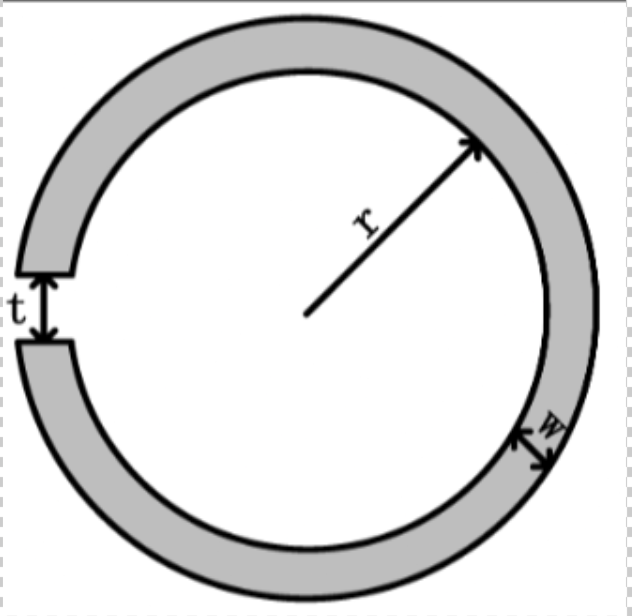
\includegraphics[width=0.2\textwidth]{Images/Single_Ring_SRR.png}
    \caption{Single Ring Circular SRR.}
    % \label{fig:SRR_circuit}
\end{figure}

\begin{figure}[h]
\centering
    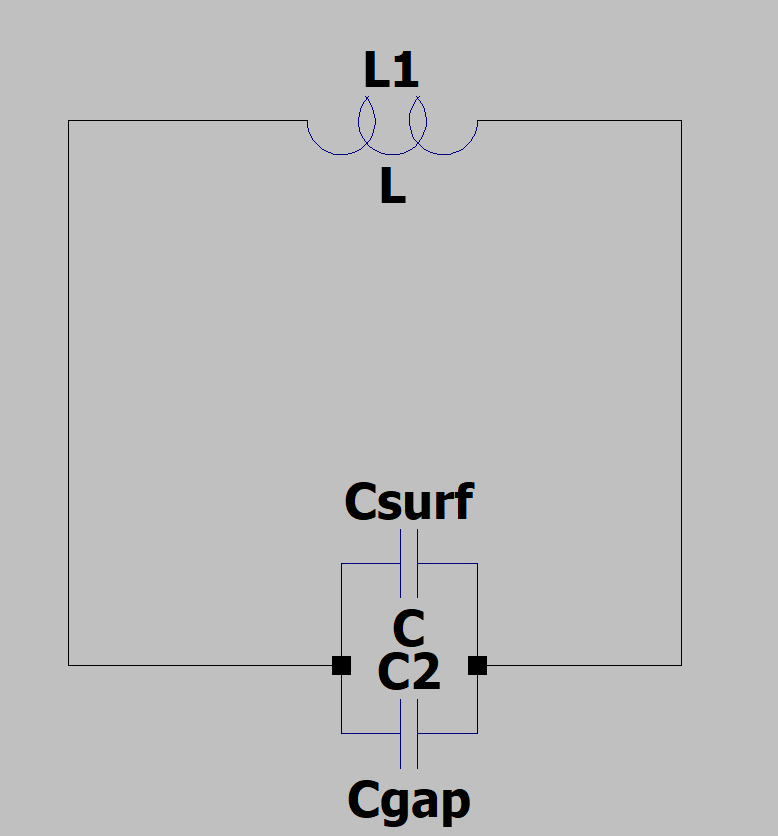
\includegraphics[width=0.2\textwidth]{Images/Single_Circular_Equivalent_model.png}
    \caption{Equivalent circuit model of a Single Ring SRR.}
    % \label{fig:SRR_circuit}
\end{figure}

\begin{equation}
    L = \mu_0 \left( R + \frac{W}{2} \right) \left( \ln\left( \frac{8\left( R + \frac{W}{2} \right)}{h + w} \right) - 0.5 \right)
    \end{equation}
    
    \begin{equation}
    C_{\text{gap}} = \varepsilon_0 \left[ \frac{wh}{t} + \frac{2\pi h}{\ln\left( \frac{2.4h}{w} \right)} \right]
    \end{equation}
    
    \begin{equation}
    C_{\text{total}} = C_{\text{gap}} + C_{\text{surface}}
    \end{equation}
\textit{Double Ring Circular SRR:}
\begin{figure}
\centering
    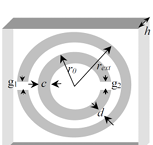
\includegraphics[width=0.2\textwidth]{Images/Double_Ring_SRR.png}
    \caption{Double Ring SRR.}
    % \label{fig:SRR_circuit}
\end{figure}

\begin{figure}
\centering
    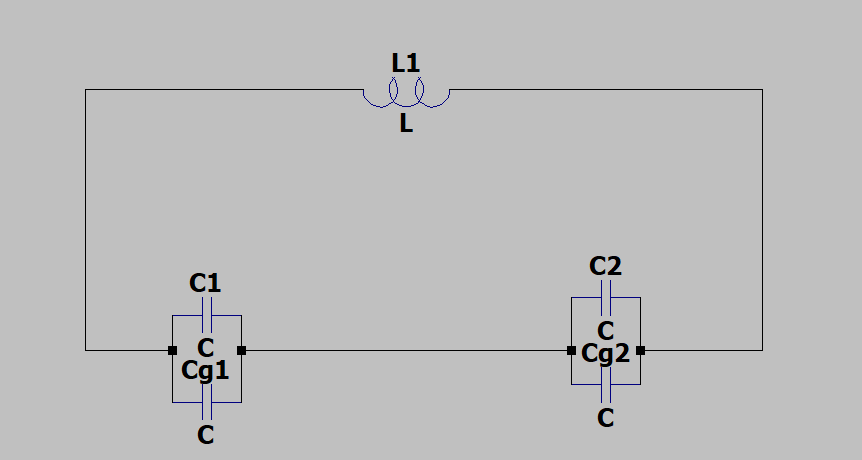
\includegraphics[width=0.3\textwidth]{Images/Double_Circular_Equivalent_modle.png}
    \caption{Equivalent circuit model of a Double Ring SRR.}
    % \label{fig:SRR_circuit}
\end{figure}
\begin{equation}
    f_{0s} = \frac{1}{2\pi \sqrt{L_r C_{eq}}} 
    = \frac{1}{2\pi \sqrt{L_r \left[ \left(2a_{\text{avg}} - \frac{g}{2} \right) C_{\text{pul}} + \frac{\varepsilon_0 c h}{2g} \right] }}
    \end{equation}
    
    \noindent
    where:
    \begin{itemize}
        \item \( f_{0s} \) is the resonance frequency
        \item \( L_r \) is the ring inductance
        \item \( C_{eq} \) is the equivalent capacitance (sum of metal-ring and gap capacitance)
        \item \( a_{\text{avg}} \) is the average radius
        \item \( g \) is the gap
        \item \( c \) is the width of the metal trace
        \item \( h \) is the substrate height
        \item \( \varepsilon_0 = \frac{1}{36\pi} \times 10^{-9} \, \text{F/m} \) (free space permittivity)
    \end{itemize}
    
    \begin{equation}
    C_{\text{pul}} = \frac{\sqrt{\varepsilon_e}}{c_0 Z_0}
    \end{equation}
    
    \noindent
    where:
    \begin{itemize}
        \item \( \varepsilon_e \) is the effective dielectric constant
        \item \( c_0 = 3 \times 10^8 \, \text{m/s} \) is the speed of light in vacuum
        \item \( Z_0 \) is the characteristic impedance of the transmission medium
    \end{itemize}
    
    \begin{equation}
    L_T = 0.00508 \, l \left( 2.303 \log_{10}\left( \frac{4l}{d} \right) - \theta \right)
    \end{equation}
    
    \noindent
    where:
    \begin{itemize}
        \item \( l \) is the conductor length
        \item \( d \) is the diameter
        \item \( \theta \) is a geometry correction constant
    \end{itemize}

\textit{Double Ring SRR with Transmission Line:}
\begin{figure}
\centering
    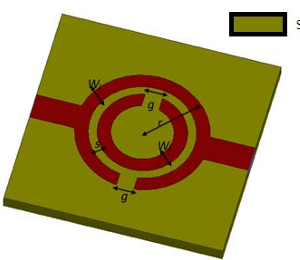
\includegraphics[width=0.25\textwidth]{Images/Double_Ring_SRR_Transmission_line.png}
    \caption{Double Ring SRR with Transmission Line.}
    % \label{fig:SRR_circuit}
\end{figure}

\begin{figure}
\centering
    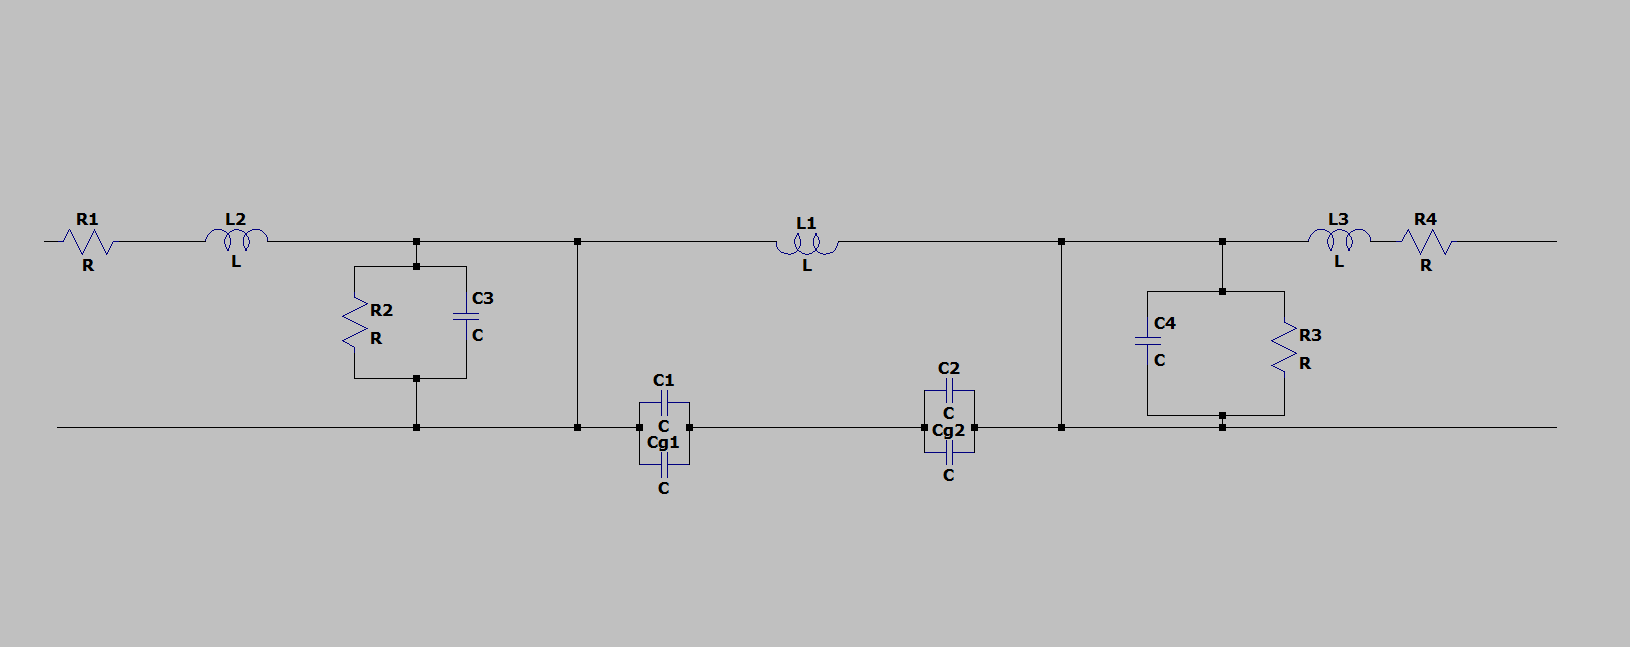
\includegraphics[width=0.25\textwidth]{Images/With_Transmission_line_Equivalent.png}
    \caption{Equivalent circuit model of a Double Ring SRR with Transmission Line.}
    % \label{fig:SRR_circuit}
\end{figure}


\begin{align}
    C_0 &= 2\pi r_0 C_{\text{pul}},  \\
    L_s &= \frac{4\pi^2 r_0^2 N^2}{1 + 0.45 \times 2 r_0},  \\
    C_c &= \frac{4 \varepsilon_0 L_s}{\mu_0},  \\
    L_0 &= \frac{C_0 \mu_0}{4 \varepsilon_0}. 
    \end{align}
    
    The resonant frequency of the fabricated CSRR can be expressed as Eq.~(5). By stretching the CSRR, an increase in \( r_0 \) causes an increase in capacitance and inductance, which ultimately causes a decrease in the resonant frequency,
    
    \begin{equation}
    f_p = \frac{1}{2\pi \sqrt{L_0 C_c}}. 
    \end{equation}

\begin{figure}[h]
\centering
    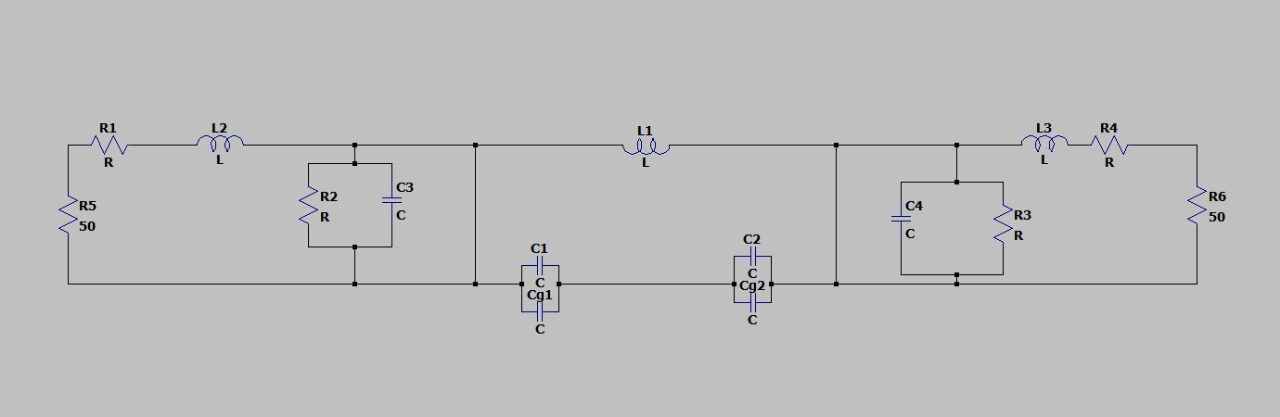
\includegraphics[width=0.5\textwidth]{Images/transmission_line_quarter_wave.jpg}
    \caption{Impedance matching using a quarter wave transformer.}
    % \label{fig:SRR_circuit}
\end{figure}

\subsection{Coupling Mechanisms}
Split Ring Resonators (SRRs) interact with electromagnetic fields primarily through two coupling mechanisms: magnetic (inductive) coupling and electric coupling. These mechanisms significantly influence their resonance behavior and are central to the design of metamaterials, filters, and sensors.

Magnetic coupling is driven by Faraday’s Law. A time-varying magnetic field from the current in one SRR induces an electromotive force (EMF) in a neighboring SRR, generating a circulating current. This mutual inductance leads to negative coupling, where the induced current opposes the original magnetic field (as per Lenz’s Law), causing the resonance frequencies to split or shift. Magnetic coupling is strongest when the SRRs are aligned with their loops facing the same direction but with gaps on opposite sides, maximizing magnetic flux linkage. This configuration is commonly used to achieve negative permeability and magnetic field confinement.

Electric coupling, on the other hand, occurs due to the interaction between the electric fields across the split gaps of SRRs. When the gaps are aligned or closely positioned, the electric field from one SRR induces a similar charge distribution across the gap of the neighboring SRR. This forms coupled electric dipoles that result in positive coupling. The fields reinforce one another, enhancing the overall electric field interaction and leading to upward resonance shifts. This effect is especially important in sensing applications, where field localization and sensitivity are crucial.

In practical configurations, both types of coupling can occur simultaneously. The relative orientation, gap alignment, and distance between SRRs can be strategically modified to fine-tune the overall coupling strength and resonance characteristics. This tunability is essential in designing components for metamaterials, reconfigurable filters, high-sensitivity sensors, and antennas.

\section{Simulation Methodology}
The numerical method used in HFSS is the Finite Element Method (FEM). In this method a structure is subdivided into many small subsections called finite elements. In HFSS these finite elements are in the form of tetrahedra. The entire collection of tetrahedra constitutes the finite element mesh. A solution is found for the fields within these tetrahedra. These fields are
interrelated so that Maxwell’s Equations are satisfied across inter-element boundaries yielding a field solution for the entire original structure. Once the field solution is found, the generalized S matrix solution is determined.
The tool also uses the automatic adaptive mesh refinement process to solve an EM problem. To set up the design, we need to create the geometry and specify material properties, boundary conditions, excitations, and the solution frequency.


\subsection{HFSS Simulation Environment Setup}
The simulation was conducted in Ansys HFSS, where boundary conditions and excitations were assigned to both 2D sheet and 3D object faces. A finite solution space was created using an air box with appropriate open boundary conditions. Mesh generation and adaptive frequency sweeps were used to ensure convergence and accurate field solutions across the desired frequency range.

\subsection{Material Properties and Model Creation}
Conductor and dielectric properties were assigned to respective parts of the model. Metal parts such as the SRR and ground plane were modeled using Perfect Electric Conductor (PEC) boundaries, and the dielectric substrate was defined with appropriate permittivity. A 3D layered geometry was created with accurate dimensions, including the SRR patterned on a dielectric slab placed above a ground plane. Ports were aligned with the transmission line ends to ensure proper excitation.

\subsection{Excitation and Boundary Conditions}
Lumped ports were placed at both ends of the transmission line to simulate input and output excitation. These ports were defined internally to the solution space with a specific impedance, allowing the extraction of modal voltages and currents. For boundary conditions, three types were primarily used:
\begin{itemize}
    \item Perfect H on surfaces perpendicular to SRR and ports to simulate magnetic wall conditions.
    \item Radiation boundary on outer faces of the air box to simulate an open environment and absorb outgoing waves,
    \item Perfect Electric Conductor (PEC) on the SRR and ground plane to model ideal metal surfaces with zero tangential electric fields.
\end{itemize}

\subsection{Post-Processing Methods}
S-parameters such as \( S_{11} \) and \( S_{21} \) were calculated from the lumped port responses to evaluate filter performance. Return loss was derived from the magnitude of \( S_{11} \), indicating the amount of signal reflected. Field distributions of electric and magnetic fields were visualized at resonance to understand coupling mechanisms and energy confinement in the SRR structure. These results helped verify the effectiveness of the filter design and identify regions of strong resonance and field enhancement.


\section{Design Methodology}
Need to design a notch filter using SRR topology there should be a sharp rejection at 5 Ghz  ith low loss outside the notch and compact dimensions.

\subsection{Substrate Selection and Microstrip Design}
The substrate acts as the dielectric medium that supports both the SRR and the microstrip transmission line. Several key parameters must be evaluated when selecting a suitable substrate:

Using \textbf{FR4} as a substrate for a Split Ring Resonator (SRR) offers several benefits:

\begin{itemize}
    \item \textbf{Low Dielectric Loss}: FR4 has low dielectric loss, which is crucial for high-frequency applications, ensuring minimal signal degradation and improved efficiency.
    \item \textbf{Thermal Stability}: FR4 provides excellent thermal stability, making it suitable for environments with varying temperatures without compromising performance.
    \item \textbf{High Dielectric Strength}: FR4 has high dielectric strength, making it reliable under higher voltages and reducing the risk of breakdown.
    \item \textbf{Stable Dielectric Properties}: FR4's dielectric properties are stable across a wide frequency range, which is important for SRRs that may operate in different parts of the spectrum.
    \item \textbf{Chemical Inertness}: FR4 is chemically inert and resistant to many solvents, ensuring consistent performance in diverse environmental conditions.
    \item \textbf{Low Loss Tangent}: The low loss tangent of FR4 minimizes energy dissipation, contributing to more efficient resonator behavior.
    \item \textbf{Ease of Fabrication}: FR4 is easy to fabricate, making it a practical choice for precision SRR structures where consistency in fabrication is essential.
\end{itemize}

Overall, FR4 offers a combination of low loss, high stability, and ease of processing, making it an ideal substrate material for SRR applications.




When selecting the metal for a Split Ring Resonator (SRR)-based notch filter, you should consider the following factors:

\begin{itemize}
    \item \textbf{High Conductivity}: The metal should have excellent electrical conductivity to minimize resistive losses at high frequencies.
    \item \textbf{Skin Effect}: The material should allow efficient current flow at the surface at high frequencies, reducing power losses.
    \item \textbf{Mechanical Properties}: The metal should have good strength and ductility for easy fabrication of precise SRR structures.
    \item \textbf{Cost-Effectiveness}: The metal should be affordable while providing the necessary performance for the application.
    \item \textbf{Corrosion Resistance}: The material should be resistant to corrosion or be easily protected with coatings to ensure long-term reliability.
    \item \textbf{Availability}: The metal should be readily available in various forms for ease of processing and sourcing.
    \item \textbf{Thermal Conductivity}: The metal should dissipate heat effectively to prevent overheating, particularly in high-power applications.
\end{itemize}

Given these factors, \textbf{copper} is often the material of choice for SRR-based notch filters. It offers excellent electrical conductivity, low resistive losses, and good thermal conductivity. Copper is also easy to fabricate and cost-effective, making it suitable for a wide range of RF applications. While it may corrode over time, its natural patina offers some protection, and additional coatings can enhance its resistance. Copper balances performance, cost, and manufacturability, making it a reliable and practical choice for SRR-based notch filters.

\subsection{SRR Topology Selection}
We need to design a Split Ring Resonator (SRR) due to its compact size, low losses, and easy integration into planar structures like PCBs. SRRs offer design flexibility, as their resonant frequency can be tuned by adjusting parameters. They provide a wide bandwidth, making them suitable for broad-frequency applications, and are effective in magnetic resonance, ideal for metamaterials. Additionally, SRRs achieve a high Q factor, making them useful for applications like filters. These advantages make SRRs an excellent choice for RF and microwave applications.


\subsubsection{Single Ring SRR}
The Split Ring Resonator (SRR) was chosen for this application due to its compact size, efficiency, and ease of integration into planar circuits. Its simple design allows for precise frequency resonance while minimizing resistive losses. The SRR's resonant frequency can be easily tuned by adjusting its geometry, making it highly adaptable for specific filtering requirements. Additionally, its high Q factor ensures sharp frequency rejection, making the SRR an ideal choice for this notch filter application.

\begin{figure}[h]
    \centering
    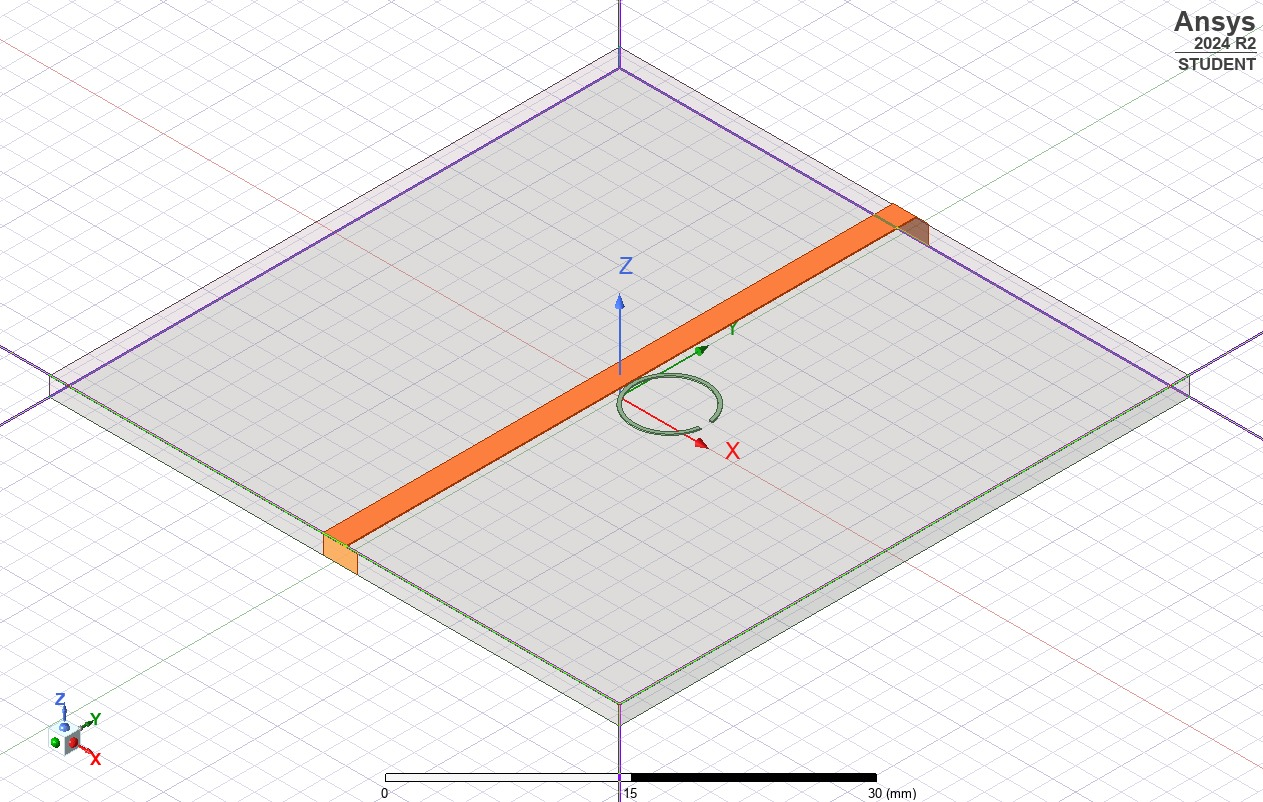
\includegraphics[width=1\linewidth]{Images/single_ring_srr_transmission_line.png}
    \caption{HFSS Simulation of single ring SRR}
    % \label{fig:enter-label}
\end{figure}

\begin{figure}[h]
    \centering
    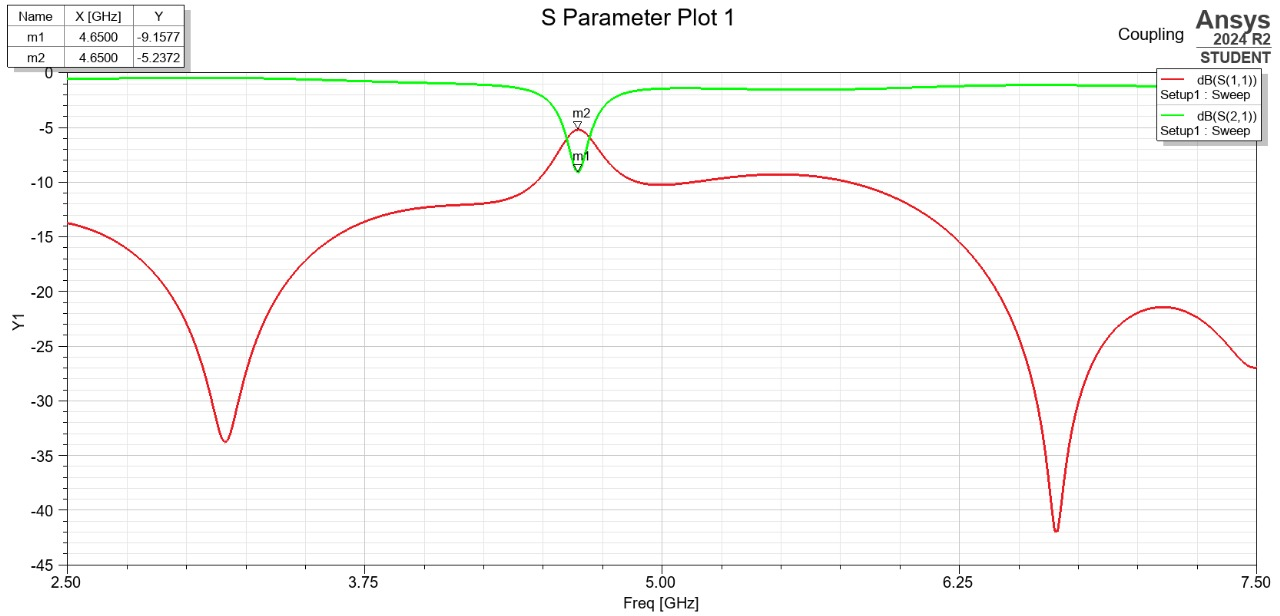
\includegraphics[width=1\linewidth]{Images/WhatsApp Image 2025-05-05 at 19.06.00_49c8992b.jpg}
    \caption{S-Parameter plot for single ring SRR}
    % \label{fig:enter-label}
\end{figure}


According to the S-parameter results, the resonant frequency specification at 5\,GHz is successfully met; however, the values of \( S_{11} \) (input reflection) and \( S_{21} \) (forward transmission) do not satisfy the required performance criteria. Hence, the coupling is not strong enough

\subsubsection{SRR with attached transmission line}
The coupling gets stronger as SRR is closer to the transmission line.

The proximity allows the stronger magnetic ( time varying magnetic field from the transmission line induced currents in the SRR more effectively)  and electric coupling (Depending on orientation, the electric field from the line can also induce polarization in the SRR, especially if gaps are aligned with the field direction).

This strong field interaction enhances energy transfer between the line and the resonator, leading to Stronger resonance effects (deeper notches in filters)

\begin{figure}
    \centering
    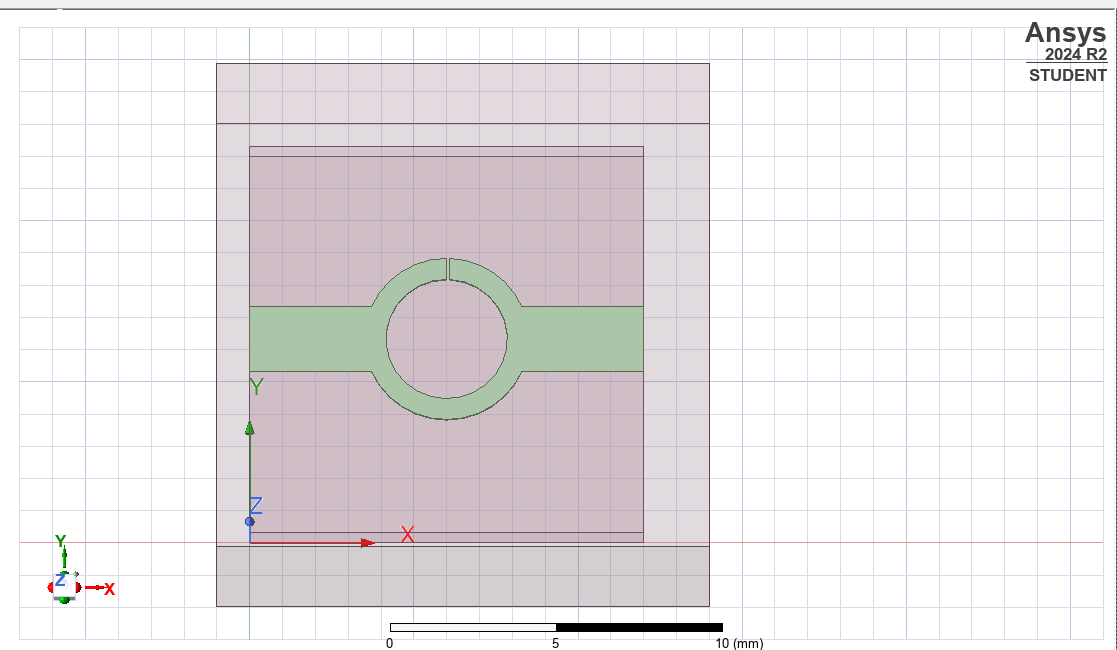
\includegraphics[width=1\linewidth]{Images/transmissionthing.png}
    \caption{HFSS of attached transmission line}
    % \label{fig:enter-label}
\end{figure}
\begin{figure}
    \centering
    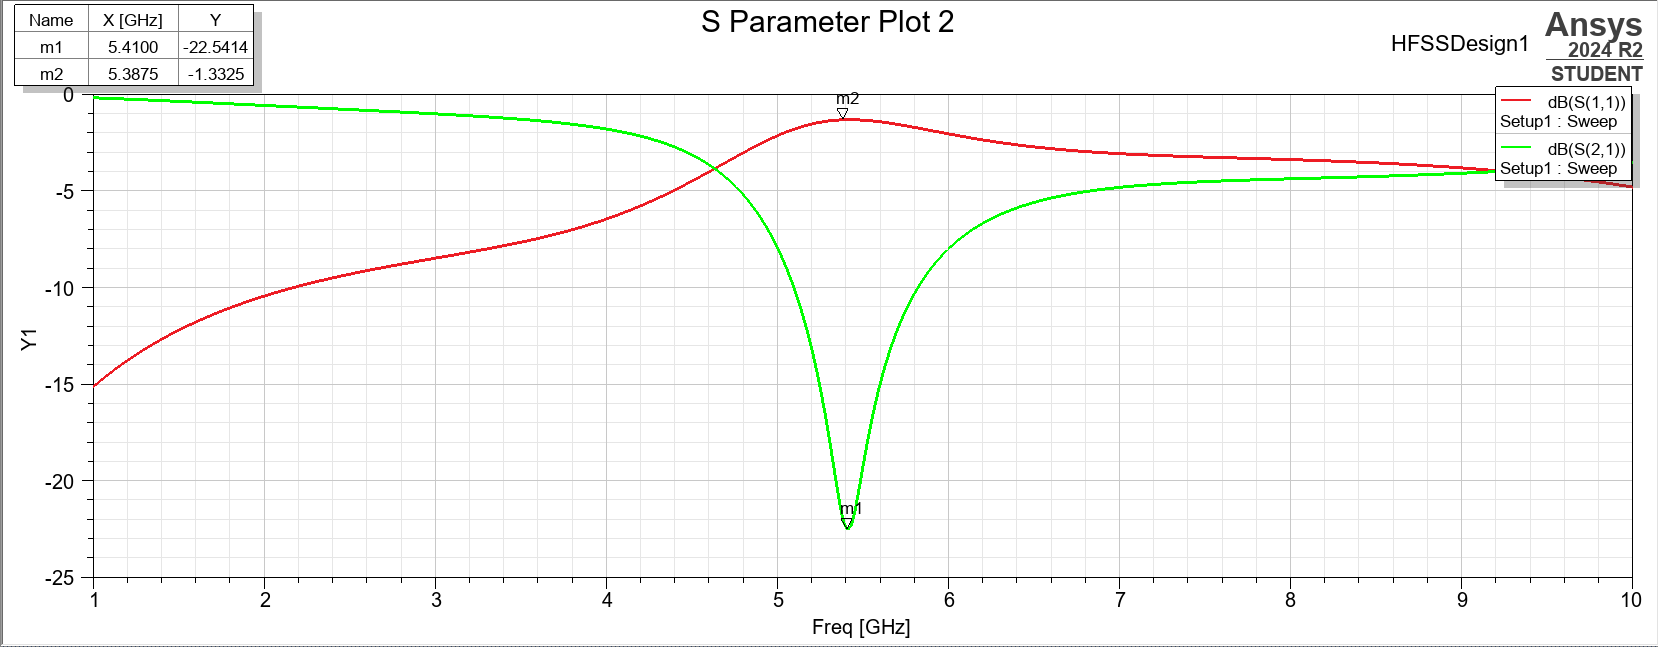
\includegraphics[width=1\linewidth]{Images/attached tranmission line.png}
    \caption{S-Parameter of the attached transmission line}
    % \label{fig:enter-label}
\end{figure}


Our goal is better coupling and better resonance frequency 


\subsubsection{Double ring SRR with attached transmission line}
In order to get better coupling we have introduced another ring inside the existing one.

\begin{figure}[h]
    \centering
    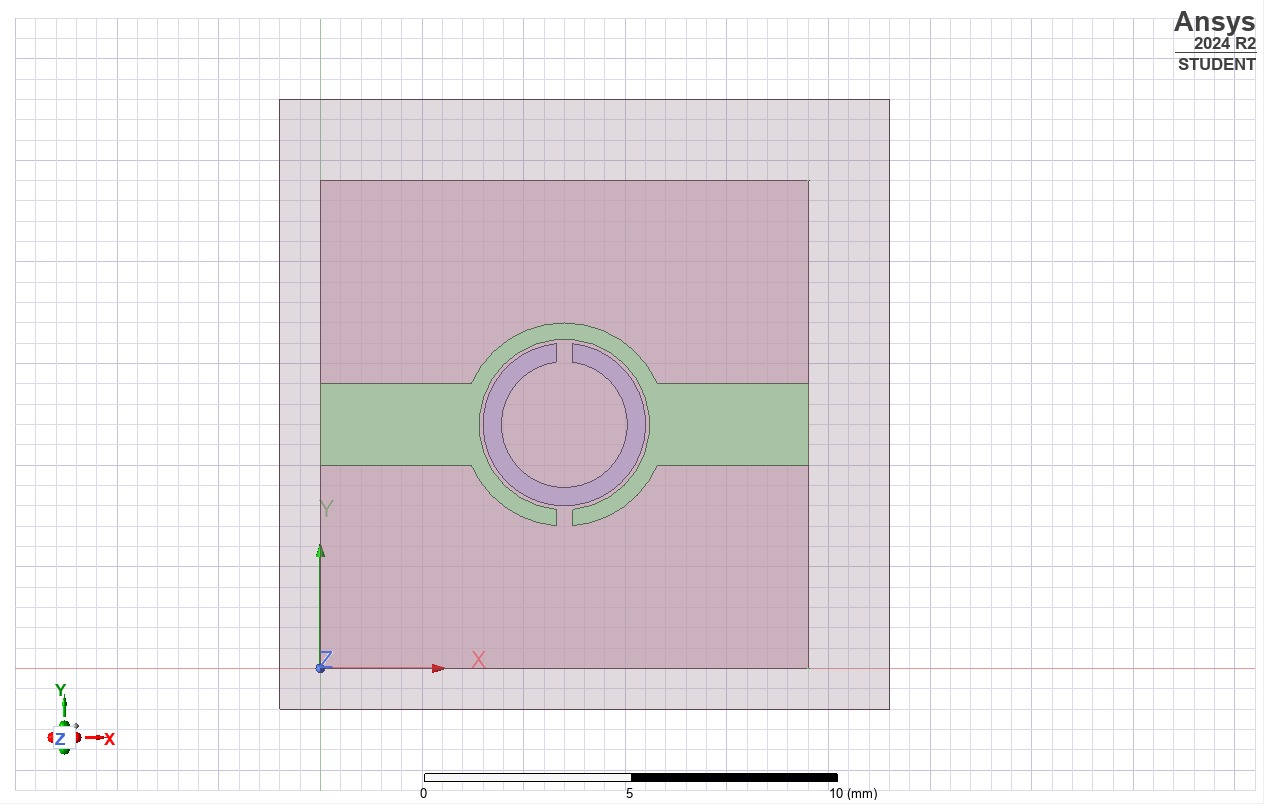
\includegraphics[width=1\linewidth]{Images/WhatsApp Image 2025-05-05 at 21.11.26_959ad83c.jpg}
    \caption{HFSS of Double ring SRR with attached transmission line}
    % \label{fig:enter-label}
\end{figure}
\begin{figure}
    \centering
    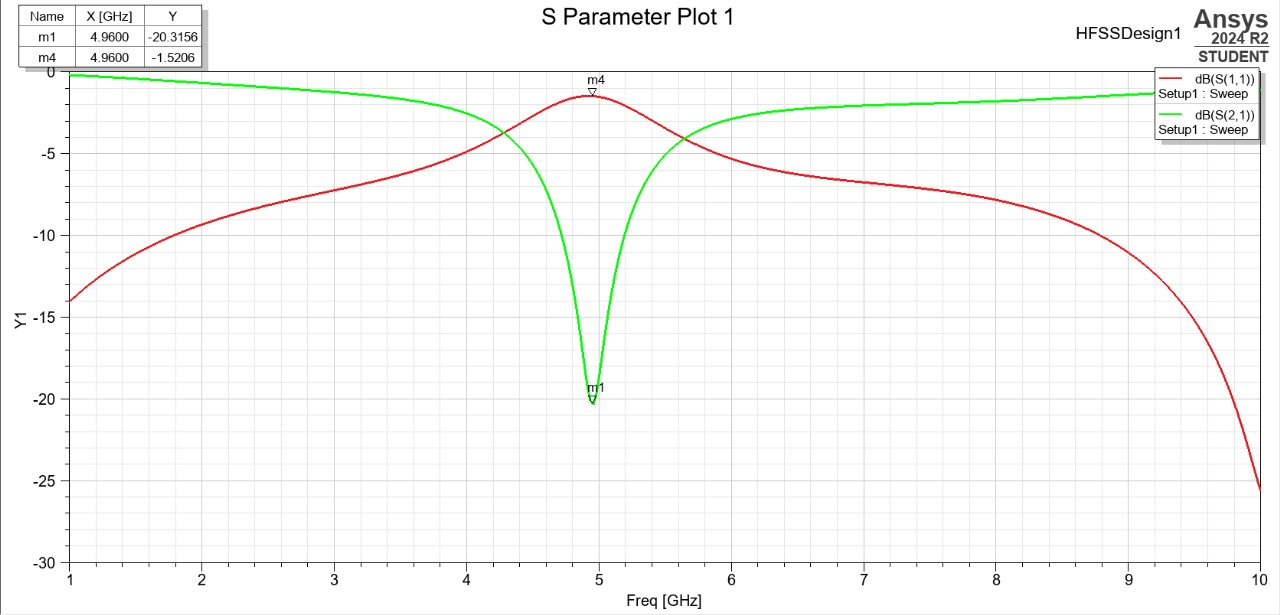
\includegraphics[width=1\linewidth]{Images/WhatsApp Image 2025-05-05 at 21.13.55_aaad92d6.jpg}
    \caption{S-Parameter of Double ring with attached transmission line}
    % \label{fig:enter-label}
\end{figure}
\begin{figure}
    \centering
    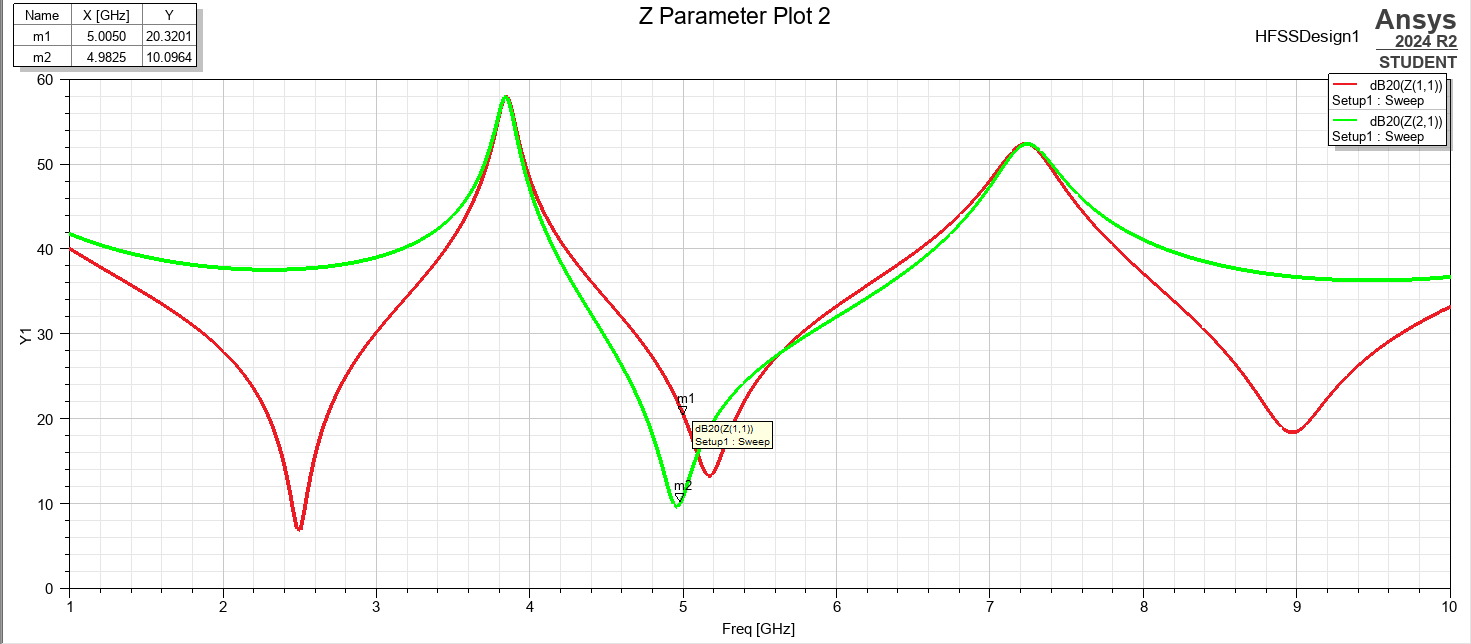
\includegraphics[width=1\linewidth]{Images/notmatchingzplot.png}
    \caption{Z-Plot of Double Ring with attached transmission line}
    % \label{fig:enter-label}
\end{figure}

As we can see in the Z-plot the impedance is not matched using this topology.
All the other specifications are satisfied.

\subsubsection{Using Quarter Wave transformer}
The impedance is not matched in the above topology so we added a quarter wave transformer to match the impedance.

\textit{\textbf{Impedance Matching using Quarter Wave Transformer}}
We can observe that the $S_{11}$ in the SRR with attached transmission line is \SI{-1.52}{\decibel}. 

\subsection*{Load Impedance Calculation}

We now calculate the load impedance ($Z_L$) at Port 1 using the following formula:

\begin{equation}
Z_L = Z_0 \left( \frac{1 + S_{11}}{1 - S_{11}} \right)
\end{equation}

First, convert $S_{11}$ from decibels to linear scale:

\begin{equation}
S_{11,\text{linear}} = 10^{\left(\frac{-1.52}{20}\right)} \approx 0.840
\end{equation}

Substituting into the formula:

\begin{equation}
Z_L = 50 \left( \frac{1 + 0.840}{1 - 0.840} \right) = 50 \left( \frac{1.840}{0.160} \right) \approx \SI{575}{\ohm}
\end{equation}

\subsection*{Reflection and Matching}

We observe that $Z_L \ne Z_0$, where $Z_0 = \SI{50}{\ohm}$. 

This implies that the load is \textbf{mismatched}, and a reflected wave exists on the transmission line. 

For \textbf{maximum power transfer}, the load should be \textbf{matched} to the transmission line, i.e., $Z_L = Z_0$, so that there is no reflection:

\[
\Gamma = 0 \quad \text{or} \quad S_{11} = 0
\]

To achieve impedance matching and eliminate reflections, we use shorted sections of transmission lines designed to transform the load impedance to match $Z_0$.

A mismatched load $Z_L$ can be properly matched to a line (with characteristic impedance $Z_0$) by inserting a transmission line $\lambda/4$ long before the load (with characteristic impedance $Z_0'$), known as a \textit{quarter-wave transformer}. $Z_0'$ is selected such that the input impedance matches the line:

\begin{equation}
Z_0' = \sqrt{Z_0 Z_L}
\end{equation}

\subsection*{Calculations:}

\begin{itemize}
    \item Load impedance, \( Z_L = \SI{22.0647}{\ohm} \)
    \item Characteristic impedance of the main line, \( Z_0 = \SI{50}{\ohm} \)
    \item Substrate height, \( h = \SI{1.6}{\milli\meter} \)
    \item Relative permittivity (dielectric constant), \( \varepsilon_r = 4.4 \)
    \item Speed of light, \( c = \SI{3e8}{\meter\per\second} \)
    \item Resonant frequency, \( f = \SI{5e9}{\hertz} \)
\end{itemize}

\subsection*{Step 1: Required Impedance of the Quarter-Wave Transformer}

\begin{equation}
Z_0' = \sqrt{Z_0 Z_L} = \sqrt{50 \times 22.0647} \approx \SI{33.21}{\ohm}
\end{equation}

\subsection*{Step 2: Effective Dielectric Constant \( \varepsilon_{\text{eff}} \)}

Assuming \( \frac{w}{h} = 1 \Rightarrow w = h \):

\begin{equation}
\varepsilon_{\text{eff}} = \frac{\varepsilon_r + 1}{2} + \frac{\varepsilon_r - 1}{2} \left( \frac{1}{\sqrt{1 + 12 \cdot \frac{h}{w}}} \right) \end{equation}
\begin{equation}
= \frac{4.4 + 1}{2} + \frac{4.4 - 1}{2} \left( \frac{1}{\sqrt{13}} \right) \approx 3.26
\end{equation}

\subsection*{Step 3: Wavelength in the Medium}

\begin{equation}
\lambda = \frac{c}{f \sqrt{\varepsilon_{\text{eff}}}} 
= \frac{3 \times 10^8}{5 \times 10^9 \sqrt{3.26}} 
\approx \SI{26.2}{\milli\meter}
\end{equation}

\subsection*{Step 4: Quarter-Wavelength Length}

\begin{equation}
l = \frac{\lambda}{4} = \frac{26.2}{4} \approx \SI{6.55}{\milli\meter}
\end{equation}

\subsection*{Final Quarter-Wave Transformer Parameters}

\begin{itemize}
    \item Required impedance, \( Z_0' = \SI{33.21}{\ohm} \)
    \item Effective dielectric constant, \( \varepsilon_{\text{eff}} \approx 3.26 \)
    \item Width of the transformer (assumed), \( w = \SI{1.6}{\milli\meter} \)
    \item Quarter-wave transformer length, \( l \approx \SI{6.55}{\milli\meter} \)
\end{itemize}
\begin{figure}[h]
    \centering
    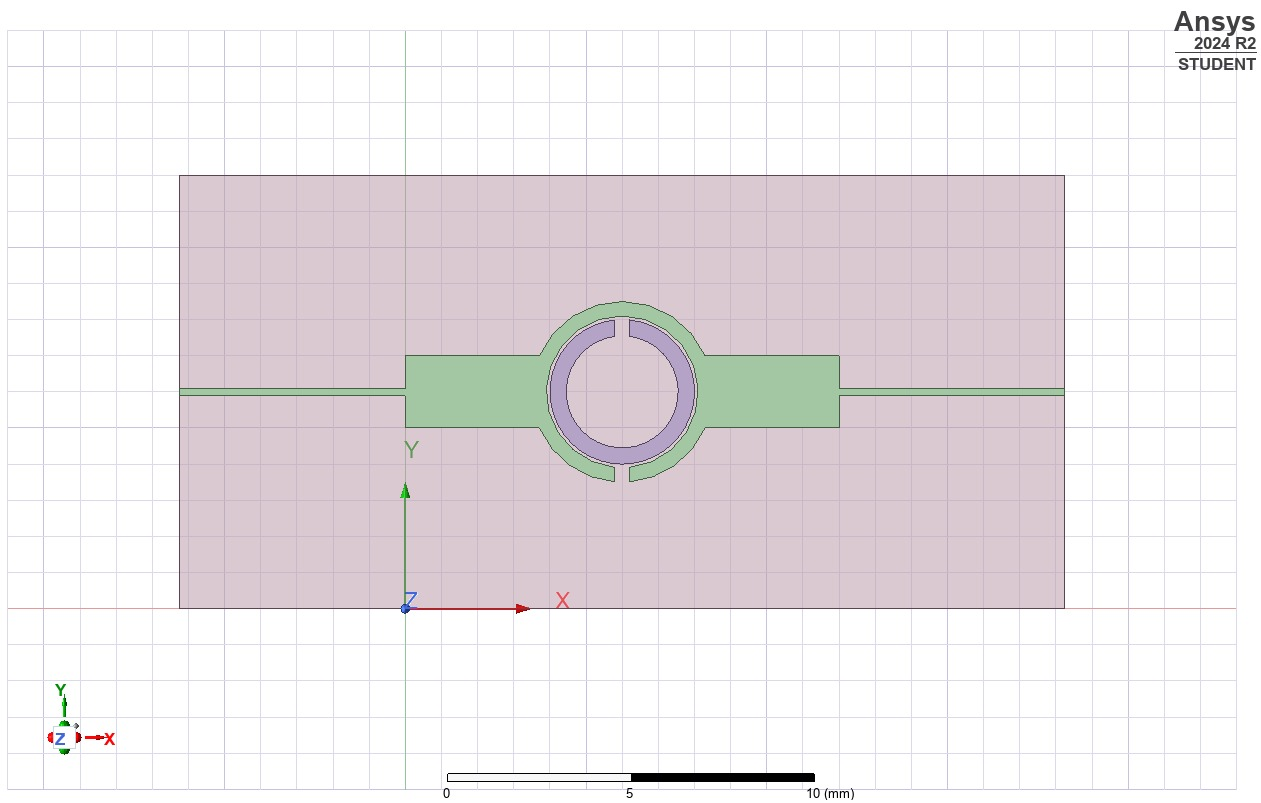
\includegraphics[width=1\linewidth]{Images/WhatsApp Image 2025-05-06 at 06.33.22_90f1b653.jpg}
    \caption{HFSS with quarter wave transformer}
    % \label{fig:enter-label}
\end{figure}
\begin{figure}[h]
    \centering
    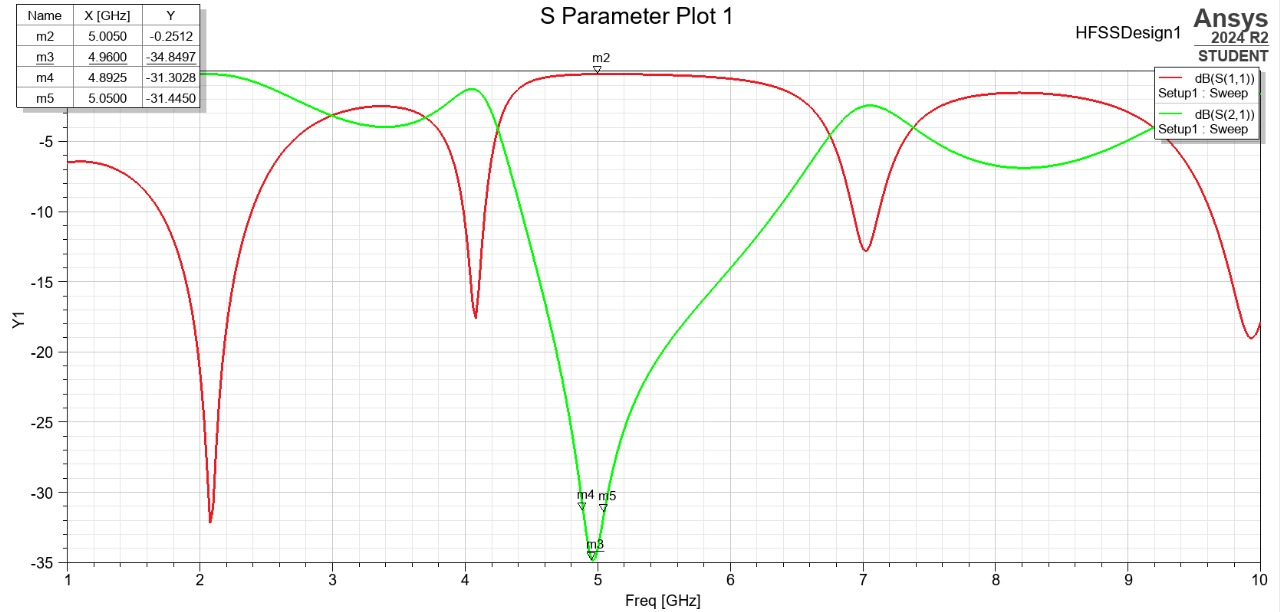
\includegraphics[width=1\linewidth]{Images/WhatsApp Image 2025-05-06 at 06.31.47_409a2904.jpg}
    \caption{S-Parameter Plot of SRR using Quarter Wave Transfomer}
    % \label{fig:enter-label}
\end{figure}
\begin{figure}[h]
    \centering
    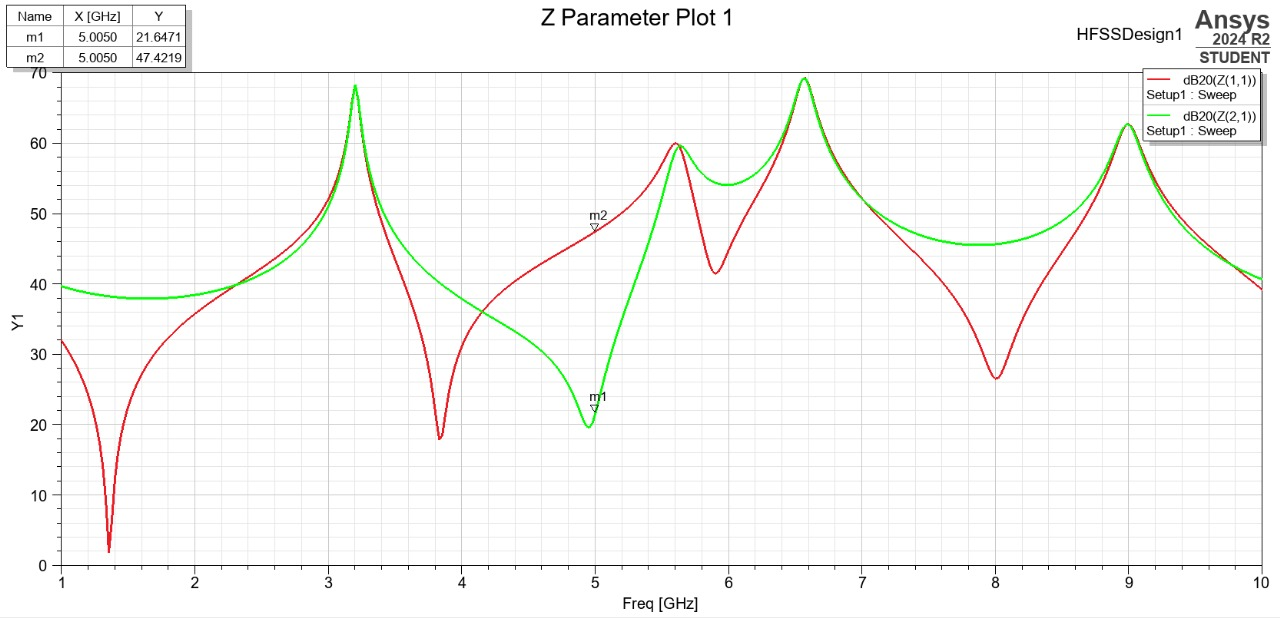
\includegraphics[width=1\linewidth]{Images/WhatsApp Image 2025-05-06 at 06.32.06_5ce3b829.jpg}
    \caption{Z-parameter Plot of SRR using Quarter Wave Transformer }
    % \label{fig:enter-label}
\end{figure}


\section{Results and Analysis}
Final Double Ring SRR Design: 5 GHz Notch Filter
\begin{figure}[h]
\centering
    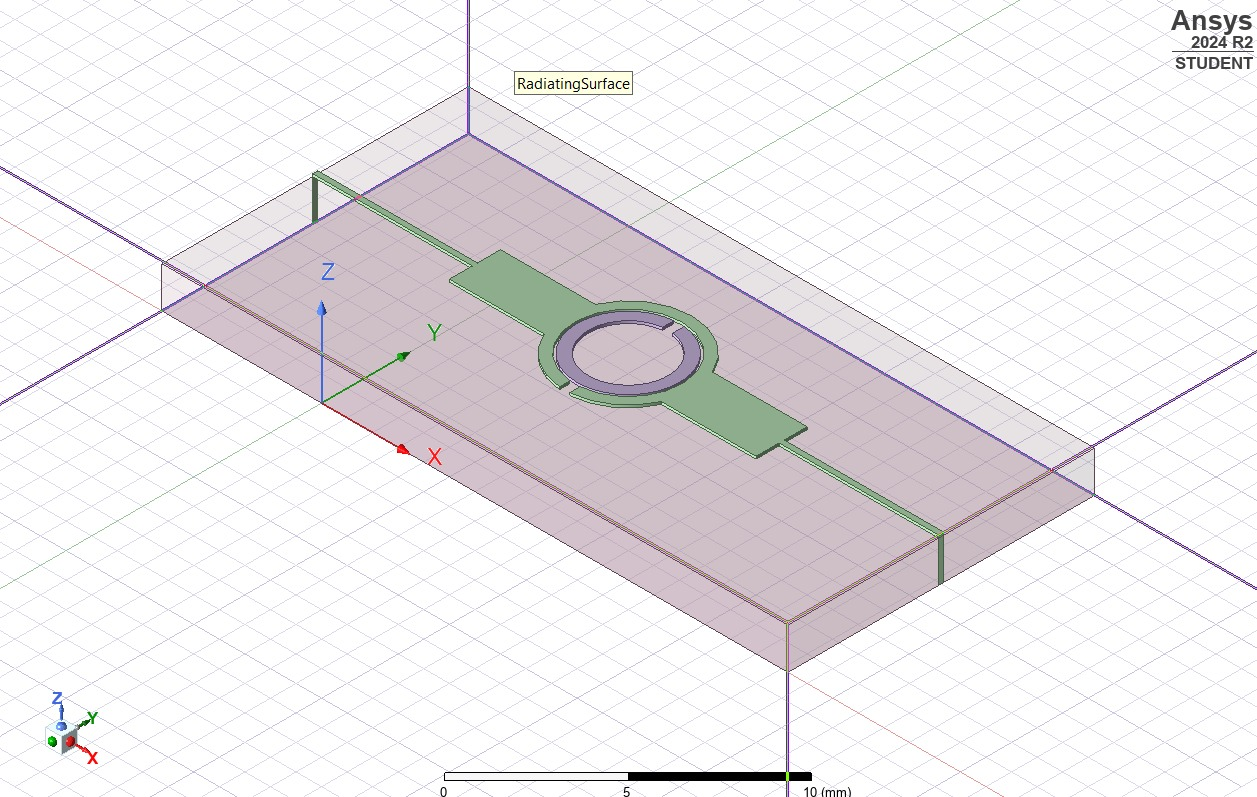
\includegraphics[width=0.5\textwidth]{Images/final_double_ring_srr.jpg}
    \caption{Final Double Ring SRR Design with Quarter Wave Transformer.}
    % \label{fig:SRR_circuit}
\end{figure}
\subsection{Resonance Frequency}

From the simulation results (S - Parameter plot), the resonant frequency is observed to be 4.96 GHz. The notch filter exhibits a sharp notch at this frequency, indicating effective filtering of signals around this frequency.
\textit{Inductance:}\\
\begin{equation}
L = \mu_0 \left( R + \frac{W}{2} \right) \left( \ln \left( \frac{8 \left( R + \frac{W}{2} \right)}{h + W} \right) - 0.5 \right)
\end{equation}
\textit{Capacitance between the Rings:}
\begin{equation}
C_{\text{gap}} = \varepsilon_0 \left[ \frac{wh}{g} + \frac{2\pi h}{\ln\left(\frac{2.4h}{w}\right)} \right]
\end{equation}
\textit{Total Capacitance:}
\begin{equation}
C_{\text{total}} = C_{\text{gap}} + C_{\text{surface}}
\end{equation}
\textit{Resonant Frequency:}
\begin{equation}
f_r = \frac{1}{2\pi \sqrt{L C_{\text{total}}}}
\end{equation}
\textit{Design Target:}
To achieve a target resonant frequency of:
\[
f_r = \SI{5}{\giga\hertz}
\]
\subsection*{Initial Parameters (Example Values):}
\begin{itemize}
    \item Mean radius of ring, \( R = \SI{1.2}{\milli\meter} \)
    \item Width of ring trace, \( W = \SI{0.4}{\milli\meter} \)
    \item Substrate thickness, \( h = \SI{0.8}{\milli\meter} \)
    \item Gap between rings, \( g = \SI{0.2}{\milli\meter} \)
    \item Ring conductor width, \( w = \SI{0.4}{\milli\meter} \)
    \item Vacuum permittivity, \( \varepsilon_0 = \SI{8.854e-12}{\farad\per\meter} \)
    \item Permeability of free space, \( \mu_0 = \SI{1.257e-6}{\henry\per\meter} \)
\end{itemize}

\subsection{Quality Factor}
The quality factor (Q-factor) is a measure of the sharpness of the resonance peak. It is defined as the ratio of the resonant frequency to the bandwidth of the filter. A higher Q-factor indicates a sharper resonance and better selectivity. The Q-factor can be calculated using the formula:
\begin{equation}        
    Q = \frac{f_o}{\Delta f}
\end{equation}
$Q = \frac{4.96}{5.05-4.8925} = \frac{4.96}{0.1575} = 31.49$

\subsection{Sensitivity}
Sensitivity is defined as the ratio of the change in resonant frequency to the change in the physical parameter (e.g., gap size, ring width). It can be calculated using the formula:
\begin{equation}        
    S = \frac{\Delta f}{\Delta X}
\end{equation}
where \( \Delta f \) is the change in resonant frequency and \( \Delta X \) is the change in the physical parameter.\\

$ S = \frac{4.96 - 4.6725}{2.6-1} = 0.1796$
\begin{figure}[h]
\centering
    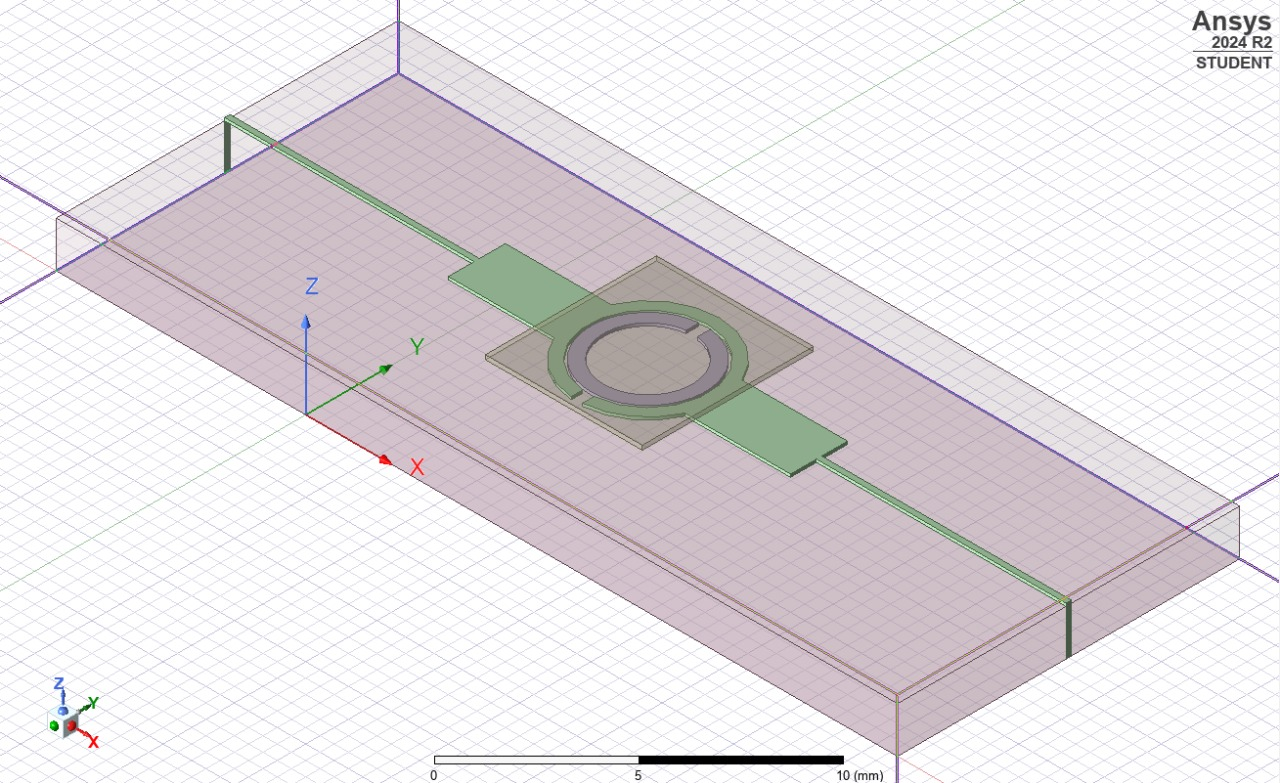
\includegraphics[width=0.5\textwidth]{Images/final_dielectric_sensitivity.jpg}
    \caption{SRR Notch filter with different analyte (Benzocyclobutene).}
    % \label{fig:SRR_circuit}
\end{figure}

\subsection{S-Parameter Results}
Final S-parameter results for the designed SRR notch filter are shown in the following figures. The S-parameters provide insight into the filter's performance, including return loss (S11) and insertion loss (S21).

We can clearly see that the S11 parameter is less than -10 dB at the notch frequency of 4.96 GHz, indicating a good return loss and effective filtering. The S21 parameter shows a significant drop at the notch frequency, confirming the filter's band-stop characteristics.

\begin{figure}[h]
\centering
    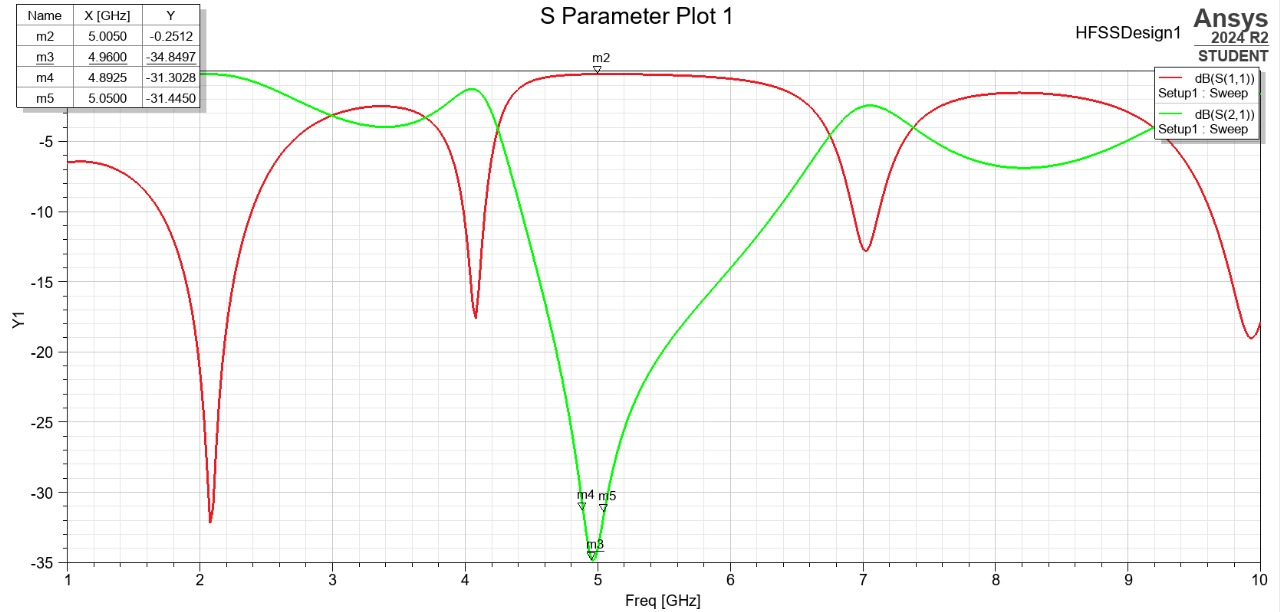
\includegraphics[width=0.5\textwidth]{Images/Fiinal_S_Param_Plot.jpg}
    \caption{S-parameter results for the designed SRR notch filter.}
    % \label{fig:SRR_circuit}
\end{figure}

\subsection{Z-Parameter Results}

Final Z-parameter results for the designed SRR notch filter are shown in the following figures. The Z-parameters provide insight into the filter's performance, including return loss (Z11) and insertion loss (Z21).

The marker m2 represents the impedance matching point, which is at 50 ohms. The Z11 parameter shows a good return loss at the notch frequency, indicating effective impedance matching. 

\begin{figure}
\centering
    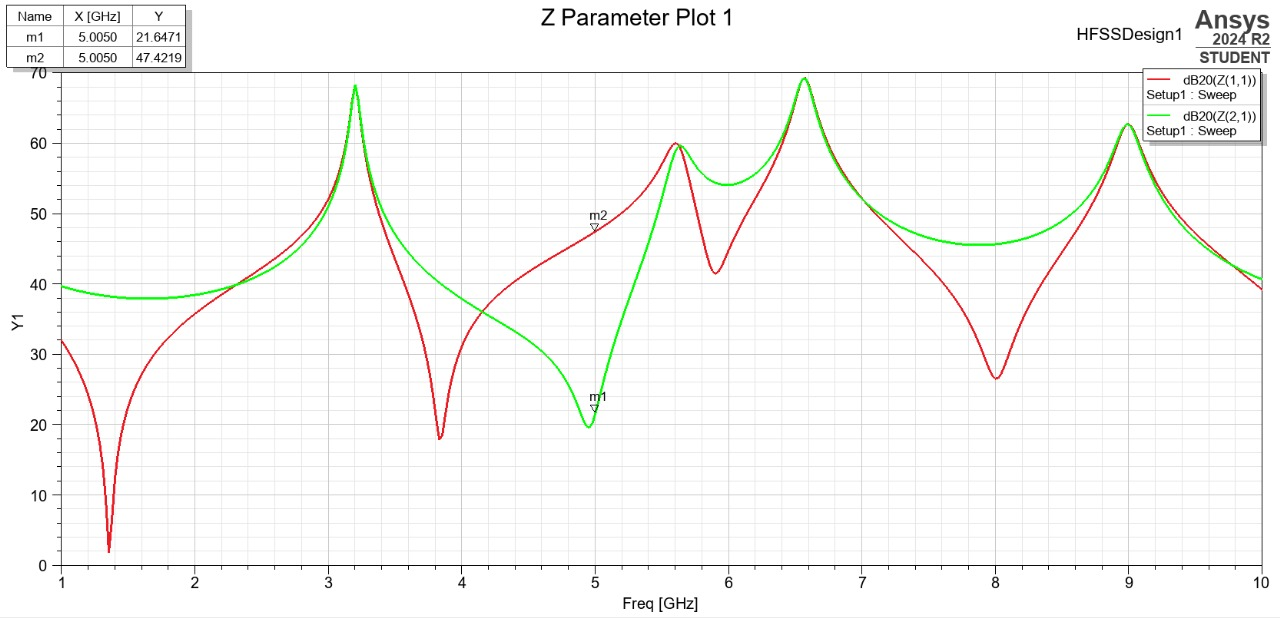
\includegraphics[width=0.5\textwidth]{Images/Final_Z_Param_Plot.jpg}
    \caption{Z-parameter results for the designed SRR notch filter.}
    % \label{fig:SRR_circuit}
\end{figure}

\subsection{Operating frequency}
The frequency at which the designed system operates is 4.96 GHz. The system is designed to operate in the 5 GHz band, which is commonly used for wireless communication systems, including Wi-Fi and Bluetooth applications. The notch filter effectively attenuates signals around this frequency, providing a means to mitigate interference from unwanted signals.

\section{Conclusion}
\subsection{Summary of Findings}
This work presents the design and simulation of a 5 GHz SRR notch filter using Ansys HFSS. The filter demonstrates a compact size, high selectivity, and effective notch characteristics. The use of a double-ring circular SRR enables miniaturization, resulting in a compact filter layout suitable for modern RF front-end applications.

\subsection{Significance of the Results}
The designed SRR notch filter is a planar structure that can be easily integrated into existing RF systems. The sharp notch and strong rejection provide excellent interference mitigation for targeted frequency bands. 

\subsection{Limitations and Future Work}
The current SRR-based notch filter design has limitations, including a fixed notch frequency without tunability, reliance on idealized simulations that do not account for real-world factors like fabrication tolerances and substrate losses, and the absence of experimental validation. Future work could focus on integrating varactors or PIN diodes to enable tunable or switchable rejection, developing multi-band configurations by combining multiple SRRs, coupling the filter with wideband antennas for system-level analysis, and exploring advanced substrates to enhance miniaturization and performance.

\subsection{HFSS Project Files:}
\href{https://github.com/MadhanSaiKrishna/Planar-Resonator-Structure}{Github Repository containing all the project files.} \\
\href{https://iiithydstudents-my.sharepoint.com/my?id=%2Fpersonal%2Fchamarthymadhan%5Fk%5Fstudents%5Fiiit%5Fac%5Fin%2FDocuments%2FSRR&ga=1}{Onedrive Folder containing all the resources gathered during the project.}  




\begin{thebibliography}{00}
\bibitem{b1} S. Dasi, S. Dasi and G. M. Rao, "Design and Analysis of a Meta Material based Nested Circular Split Ring Resonator for Terahertz Applications," 2022 International Conference on Automation, Computing and Renewable Systems (ICACRS), Pudukkottai, India, 2022, pp. 178-181, doi: 10.1109/ICACRS55517.2022.10029069.

\bibitem{b2}C. Saha and J. Y. Siddiqui, "A comparative analyis for split ring resonators of different geometrical shapes," 2011 IEEE Applied Electromagnetics Conference (AEMC), Kolkata, India, 2011, pp. 1-4, doi: 10.1109/AEMC.2011.6256871.

\bibitem{b3}
Band-stop filter design based on split ring resonators loaded on the microstrip 
transmission line for GSM-900 and 2.4 GHz ISM band https://dergipark.org.tr/en/download/article-file/1034899

\bibitem{b4}
Analysis and Design of Direct Coupled Metamaterial Filters for Wireless Communication


\bibitem{b5}
Compact Microstrip Band Stop Filter Using SRR and CSSR: Design, Simulation and Results

\bibitem{b6}
Design and Analysis of a Meta Material based Nested Circular Split Ring Resonator for Terahertz Applications 

\bibitem{b7}
Electromagnetic Metamaterial Based Sensor Design for Chemical Discrimination 

\bibitem{b8}
FEM Modelling of Split Ring Resonator Based Metamaterials for UWB Notch Filter Applications

\bibitem{b9}
DESIGN AND ANALYSIS OF SQUARE SPLIT RING RESONATOR METAMATERIAL FOR MICROWAVE FREQUENCY RANGE

\bibitem{b10}
Metamaterial based CPW band stop filter for WLAN application 

\bibitem{b11}
Utilization of Split Ring Resonator for Compact Narrowband Microstrip Bandpass Filter
\end{thebibliography}

\end{document}
